\chapter{ Аналитический раздел}
\label{cha:analysis}


\section {Понятие манги.}

Страницы манги - это олицетворение сценария. Сценарий отражает события,
характеры персонажей, описывает места действий, отражает разбиение на страницы
и кадры. Разбиение на кадры принято называть раскадровка. Процесс раскадровки
зависит от типа сюжета: комедийный, мелодраматический или трагический требует
своего способа постановки сцен. Раскадровка - это основа будующего кадра (фрейма).
Внутри каждого фрейма располагаются баллоны, содержащие диалоги. При
отрисовке фреймов существует правило "динамичной сцены". 

На одной странице движение персонажа обуславливается сохранением направления перемещения. При
изображении движения внутри кадра используются вихри, описывающие направление
движения и следа, отображающего положение на предудещем шаге бледнее, чем
на текущем, в рамках одного фрейма (Рисунок 1.1).

\begin{figure}[ht!]
	\centering{ 
		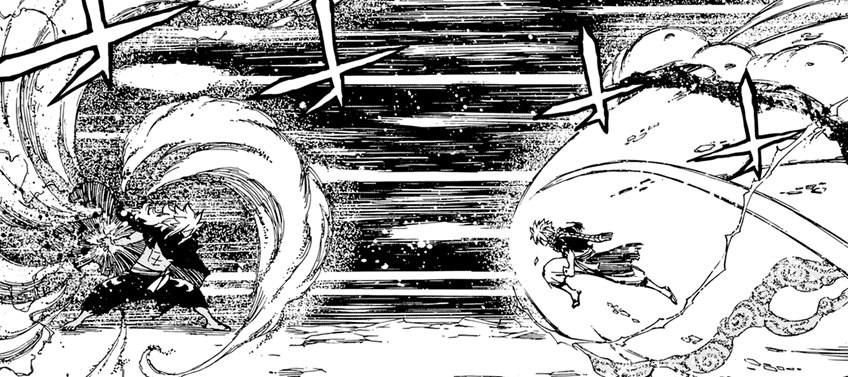
\includegraphics[width=0.5\textwidth]{img/1_1.jpg}
		\caption{Пример движения внутри фрейма.}}
\end{figure}


 Для отображения мимики и ее изменения используются
крупные планы, для композиции общие, для второстепенных событий
средние (Рисунок 1.2). 


\begin{figure}[ht!]
	\centering{ 
		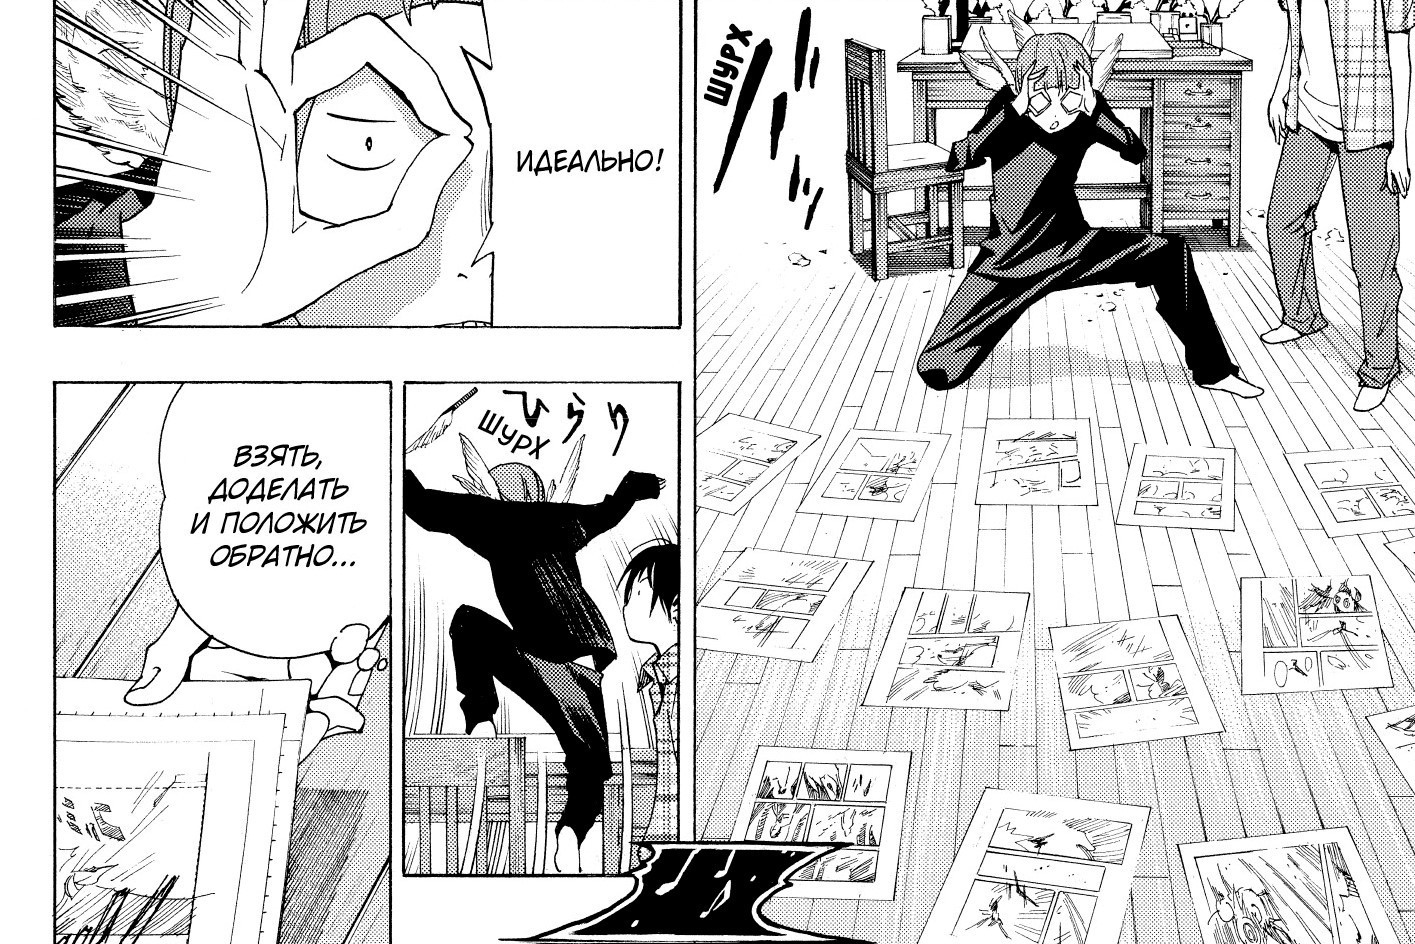
\includegraphics[width=0.5\textwidth]{img/1_2.jpg}
		\caption{Пример отображения мимики и второстепенного плана.}}
\end{figure}

Панорамные (горизонтальные или вертикальные) кадры дают возможность
выразительно показать движение, поскольку в движении главное - большая амплитуда (Рисунок 1.1).
Если действие должно изображаться в разных местах, с разными персонажами
в одно и то же время, персонаж придается воспоминаниям либо мечтает, изменяется
объект или оформление страницы, которые подчеркивают факт, что события все таки
отделены (например фоновый цвет страницы может быть не белым, а черным).


Предметы заднего плана всегда имеют меньшую детализацию и изображаются либо
более тонким контуром, либо более плотной массой, в отличие от деталей переднего
плана. Тени на переднем плане более плотные и могут быть черными, в то время как
на фоне они будут сделаны скринтоном (особый вид штриховки). Линии - попадающие под свет более тонкие, чем те, что находятся в тени. Тени бывают двух видов:
рисующие объем поверхности и падающие (которые отбрасывают одни предметы на
плоскости других (Рисунок 1.3). 


\begin{figure}[ht!]
	\centering{ 
		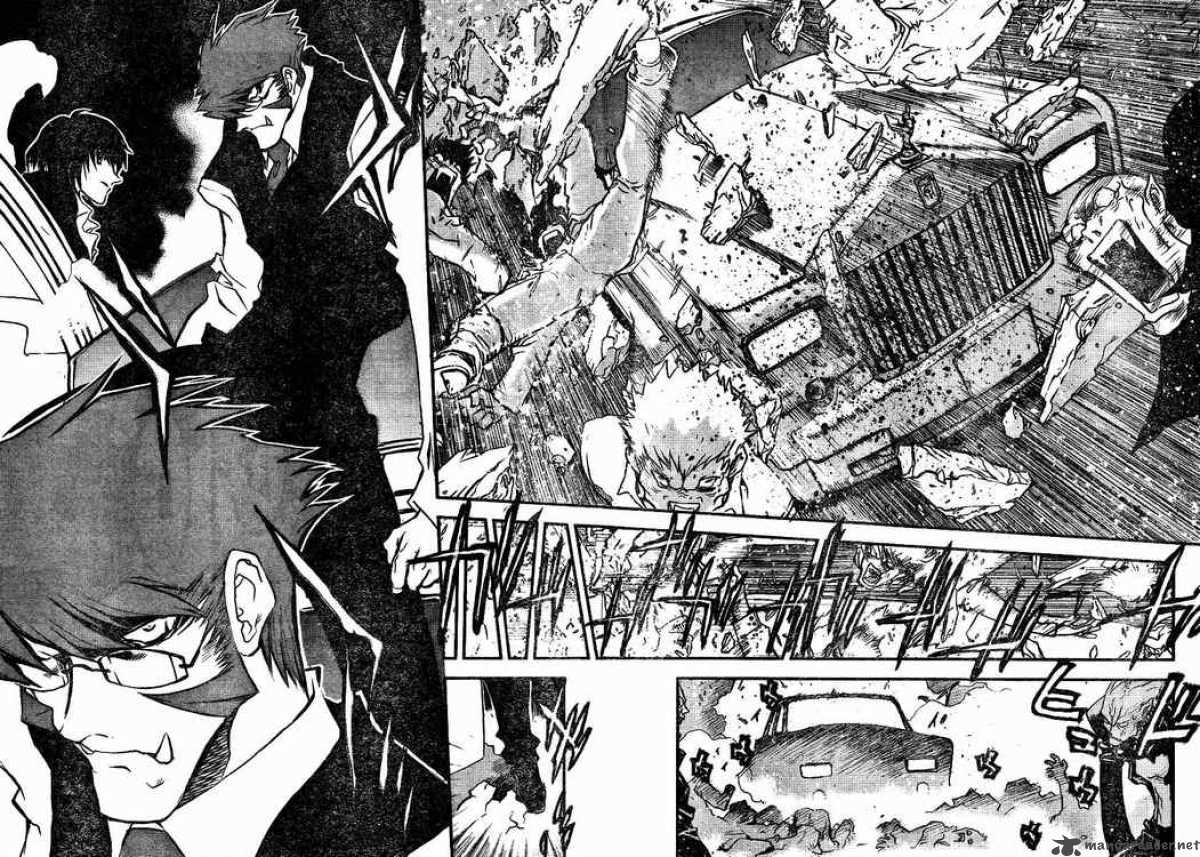
\includegraphics[width=0.5\textwidth]{img/1_4.jpg}
		\caption{Пример передачи объемных поверхностей.}}
\end{figure}

\section{Описание методов, решающих поставленную проблему.}
Существует несколько методов, решающих проблему колоризации графической новеллы. Однако, среди них всех можно выделить два основных:

\begin{enumerate}
	\item колоризация изображения с использованием цветовых подсказок;
	\item колоризация изображения, основанная на опорном цветном изображении с использованием графика соответствия и методов квадратичного программирования.
\end{enumerate}


Программное решение проблемы колоризации с использованием 
цветовых подсказок делится на основные этапы:
\begin{enumerate}
	\item считывание цветовых подсказок, рекомендуемых для закраски;
	\item распознавание на еще не закрашенном изображении граничных областей;
	\item принятие ограничений и допущений, касаемых незамкнутых областей;
	\item выделение граничных областей;
	\item на выделенных граничных областях распознавание типов штриховки, вычисление плотности штриховки;
	\item вычисление необходимой интенсивности закраски для цветового акцента относительно рассматриваемой области;
	\item колоризация изображения по областям.
\end{enumerate}

Программное решение проблемы колоризации изображения с использованием опорного цветного изображения, графика соответствия и квадратичного программирования состоит из следующих этапов:
\begin{enumerate}
	\item загрузка шаблонной модели колоризованной манги;
	\item распознавание на еще не закрашенном изображении граничных областей;
	\item принятие ограничений и допущений, касаемых незамкнутых областей;
	\item выделение граничных областей;
	\item распознавание на шаблонной модели граничных областей, считывание закраски;
    \item на выделенных граничных областях колоризованного шаблона и черно-белого
изображения распознавание типов штриховки, вычисление плотности штриховки;
   \item перенос закраски с модели на черно-белое изображение.
\end{enumerate}

\subsection{Подготовка к закраске. Выделение областей колоризации.}

 Для колоризации манги на начальном этапе необходимо
определить области закраски, тоесть выделить контур рисунка. Выделение контура, как и выделение границ изображения относится к поиску объектов и их выделению, основанному на алгоритмах, которые определяют точки цифрового изображения, резко
изменяющие яркость и имеющие неднородности.  Границы и края областей сильно связаны, так как часто существует сильный перепад яркости на границах областей. Обнаруженные края бывают разорванными. Но чтобы выделить объект на изображении, нужны замкнутые границы области. Для незамкнутых областей используют дополнение: соединяются концы линий, вычисляется площадь полученной фигуры (объемлющая оболочка), выбирается область равная максимальному размеру объемлющей оболочки. Так как объемлющая оболочка - это абстрактно замкнутая область, которая может не учитывать специфику границ, используется функция ошибки. 

 Область контура инициализируется функцией:
\begin{equation}
v(s) = [x(s), y(s)], s \in [0, 1]
\end{equation} 
Данная функция "перемещается" по пространсвенной области изображения с целью минимизации энергии перепадающей интенсивности, до тех пор, пока не будет подобрана идеальная область изображения. 
Энергия описывается следующим образом:
\begin{equation}
E = \int_{0}^{1} \frac{1}{2} |\alpha(v\prime(s))^2 + \beta(v\prime\prime(s))^2 + Eext(v(s))|ds
\end{equation}
Где Eext - выходящая энергия (тоесть энергия идущая из внутренней области во внешнюю):
\begin{equation}
Eext = -[\nabla I(x, y)^2]
\end{equation}
$\alpha, \beta$ - весовые коэффициенты, которые численно определяют замкнутость и стянутость относительно центральной точки.
Функция E также еще обозначается как Eint - входящая энергия. Минимальное значение входящей энергии в контур, будет одназначно задавать контур, аппроксимирующий искомую область.
$\nabla I(x, y)$ - дивергенция интенсивности цвета границы.

Результат выделения границ представлен на Рисунок 1.4.

\begin{figure}[ht!]
	\centering{ 
		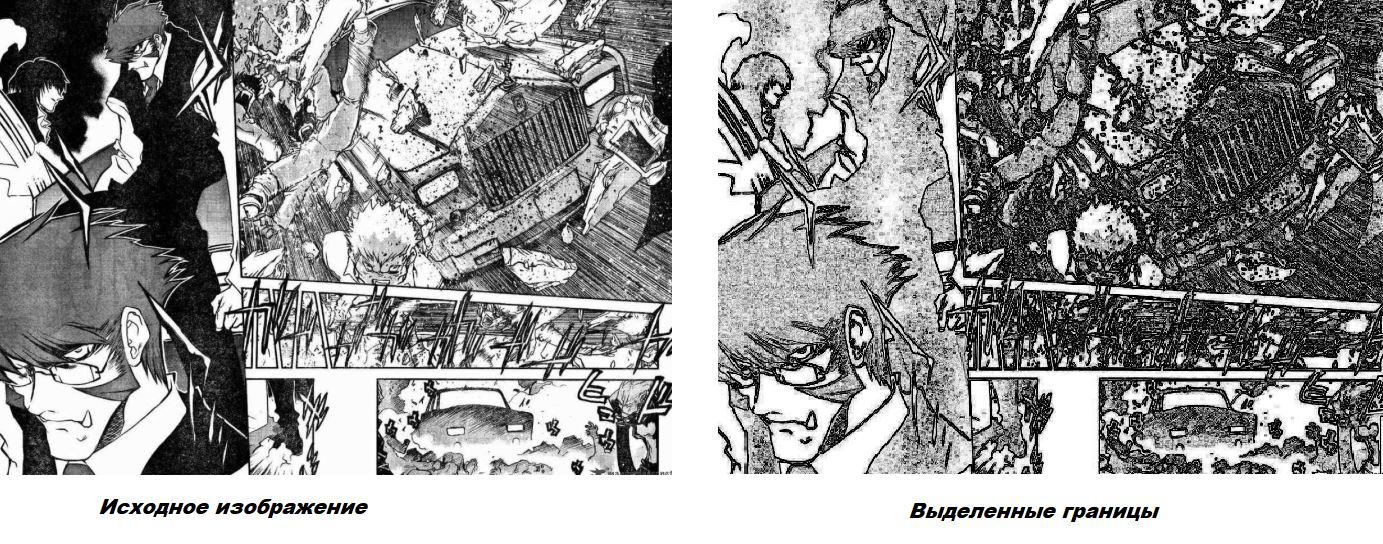
\includegraphics[width=0.7\textwidth]{img/1_5.jpg}
		\caption{Пример выделения границ.}}
\end{figure}

\subsection{Подготовка к закраске. Выделение областей колоризации. Нейросетевой метод.}

Для сегментации изображения - выделения границ так же используют нейронную сеть U-Net.
U-Net — это архитектура свёрточной нейронной сети, предназначенная для сегментации изображений.
Архитектура сети представляет собой последовательность слоёв свёртка и пулинг, которые сначала уменьшают пространственное разрешение картинки, а потом увеличивают его, предварительно объединив с данными картинки и пропустив через другие слои свёртки. Таким образом, сеть выполняет роль своеобразного фильтра. Структура сети представлена на Рисунок 1.5.

\begin{figure}[ht!]
	\centering{ 
		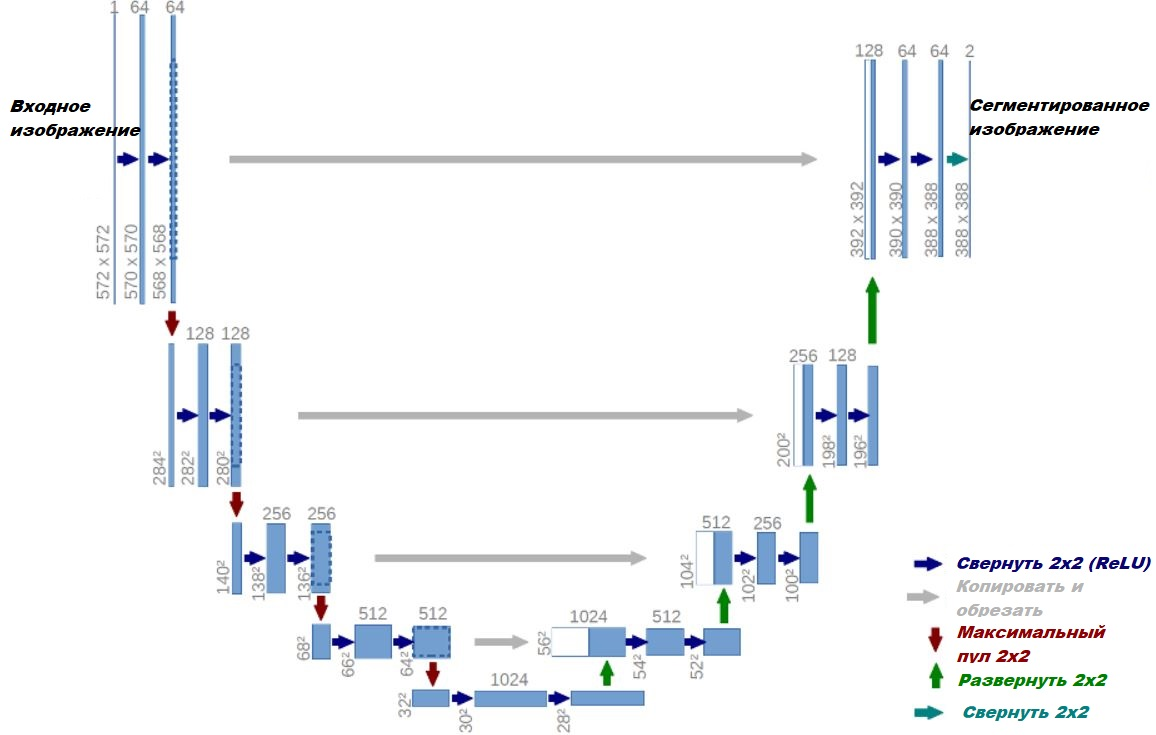
\includegraphics[width=0.7\textwidth]{img/1_7.jpg}
		\caption{Архитектура U-Net.}}
\end{figure}

Сеть содержит сжимающий путь (слева) и расширяющий путь (справа), поэтому архитектура похожа на букву U, что и отражено в названии. На каждом шаге мы удваиваем количество каналов признаков.

Сжимающий путь похож на типичную свёрточную сеть, он содержит два подряд свёрточных слоя 3x3, после которых идет слой ReLU и пулинг с функцией максимума 2×2 с шагом 2.

Каждый шаг расширяющего пути содержит слой, обратный пулингу, который расширяет карту признаков, после которого следует свертка 2x2, которая уменьшает количество каналов признаков. После идет конкатенация с соответствующем образом обрезанной картой признаков из сжимающего пути и две свертки 3x3, после каждой из которой идет ReLU. Обрезка нужна из-за того, что мы теряем пограничные пиксели в каждой свертке. На последнем слое свертка 1x1 используется для приведения каждого 64-компонентного вектора признаков до требуемого количества классов.

Всего сеть имеет 23 свёрточных слоя.

Для обучения сети, считается мера Жаккара, которая показывает меру сходства — применимо к решению задачи выделения границ, показывает меру площади правильно отмеченных сегментов (отношение площади пересечения к площади объединения). 

Мера Жаккара — бинарная мера сходства, безразмерный показатель сходства сравниваемых объектов. 

\begin{equation}
K_j = \frac{a}{a + b - c}
\end{equation}


Где a - количество видов на первой пробной площадке, b - количество видов на второй пробной площадке, c - количество общих видов на первой и второй площадках.

Пусть A - это множество, описывающее количество видов с первой пробной площадки, B - множество, описывающее количество видов со второй пробной площадки, $n(A)$, $n(B)$ - мера множества А и В соответсвенно. 

Тогда, используемая в U-Net мера различия выражается так:

\begin{equation}
F_{1,-1} = 1 - \frac{n(A \cap B)}{n(A) + n(B) - n(A \cap B)} - \frac{n(A \cup B) - n(A \cap B)}{n(A \cup B)}
\end{equation}


\section {Колоризация изображения с использованием цветовых подсказок.}

Автоматизированный метод раскраски манги с использованием цветовых подсказок решает задачу колоризации графических
монохромных изображений.

Данный метод использует U-Net (для выделения границ) и архитекуру GAN (генеративная нейронная сеть). 
GAN представляет собой алгоритм машинного обучения без учителя, построен на комбинации двух нейронных сетей: генеративной, которая занимается генерацией образов, и, дискриминативной, которая отличает правильные ("подлинные") образцы от неверных. 

На Рисунок 1.6 представлена общая структура  метода.

\begin{figure}[ht!]
	\centering{ 
		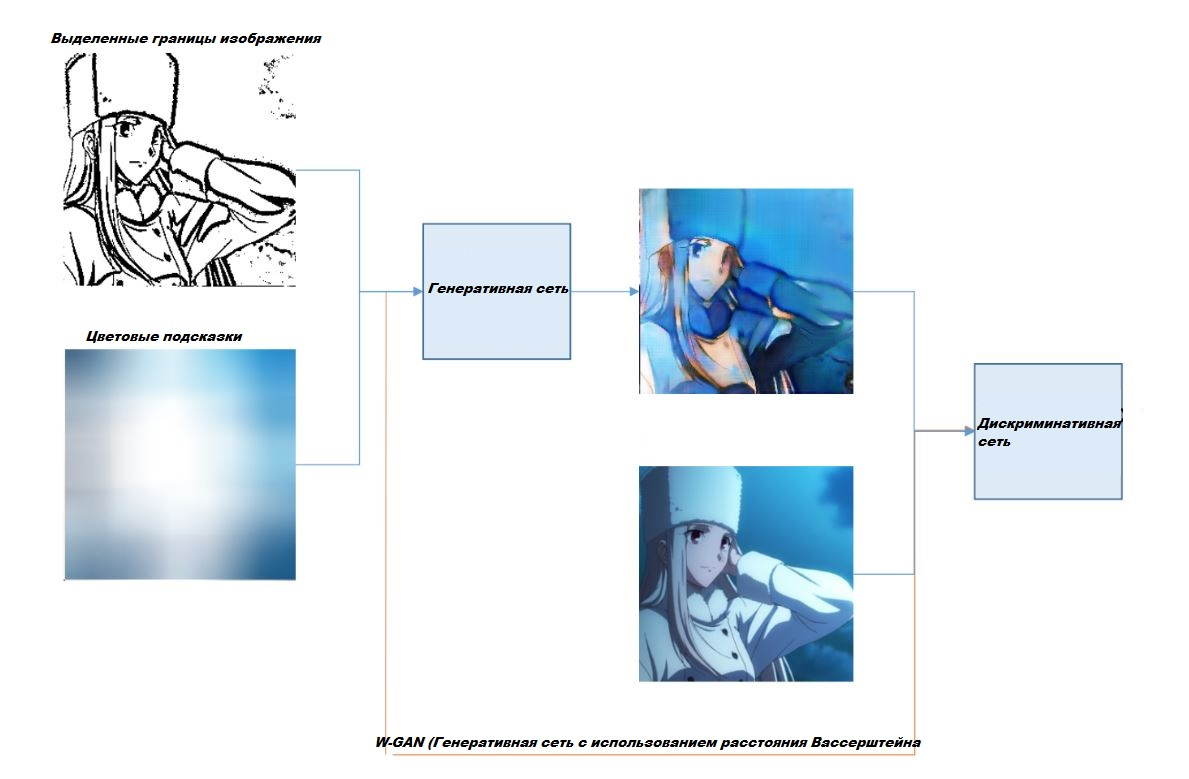
\includegraphics[width=0.8\textwidth]{img/1_8.jpg}
		\caption{Структура метода колоризации с использованием цветовых подсказок.}}
\end{figure}

GAN включает в себя 2 нейронные сети: генеративную $G(z; \theta_g)$ и дискриминативную $D(x; \theta_d)$. $G(z; \theta_g)$ - сеть, которая оценивает вероятность равномерного распределения $p_g(x)$ по $x$ входным данным, $z$ - это входные выделенные границы изображения. Сеть $D(x; \theta_d)$ выступает в роли классификатора - выносит суждение о том, является ли изображение сгенерированным или оно из реального набора.  $G(z; \theta_g)$ - используется для прямой генерации из эскиза и цветовой подсказки цветного изображения внутри аналогично построенной U-Net сети. Дискриминатор В U-Net - $D(x; \theta_d)$ реализован, как двухклассовый классификатор. Для обучения двух нейронных сетей определена потеря при классификации как :

\begin{equation}
\nabla \theta_d \frac{1}{m} \sum\limits_{i = 1}^m (log(D(x^i; 
\theta_d)) + log(1 - D(G(z^i; \theta_d); \theta_d)))
\end{equation}

$D(x; \theta_d)$ быстро обучается отличать реальную картинку от мусора, вызываемого $G(z; \theta_g)$. Процесс генерации более подходящих изображений, корреляции ошибки генератора, и постепенного инкрементирования значения ошибки предствлено на графике Рисунок 1.7. 

\begin{figure}[ht!]
	\centering{ 
		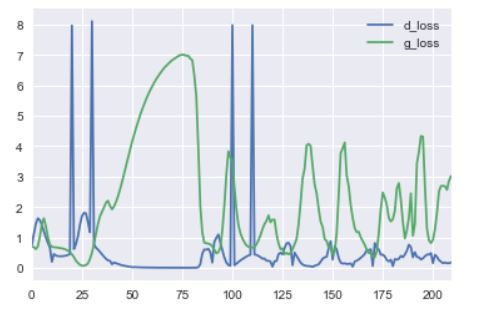
\includegraphics[width=0.5\textwidth]{img/1_6.jpg}
		\caption{Кривые потерь для генеративной и дискриминативной сетей.}}
\end{figure}

Для получения более гладкого изображения, реализации плавных цветовых переходов,  перед уровнем линейного предсказания, до использования дискриминатора, применяется формула тотального сглаживания, выступа, для каждого пиксела внутри строки (меняется координата y).


\begin{equation}
V(y) = \sum_{i,j} \sqrt{|y_{i+1, j} - y_{i,j}|^2 + |y_{i, j+1} - y_{i, j}|^2}
\end{equation}

Ввиду полученного графика (Рисунок 1.7) потерь, можно также сделать вывод, о том, что на практике трудно балансировать тренировку генератора и дискриминатора.  Если дискриминатор слишком силен,
его потеря скоро станет нулевой, а потеря генератора продолжит инкрементироваться. Для решения этой проблемы используется балансировка методом Вассерштейна. Тогда итоговая функция потери дискриминатора и генератора будет определена по формуле 1.8. W-расстояние (расстояние Вассерштейна) может быть аппроксимировано отрицательным значением, которое интерпритируется как декремент потери дискриминатора. Изображениям более высокого качества будет соответсвовать меньшее значение W-расстояния. W-расстояние является случайной величиной, распределенной по показательному закону. 

\begin{equation}
L(D) = E_{x~p_g}[D(x)] +  \lambda E_{x~p_\xi}[||\nabla D(x)||_{p_g} - 1] ^ 2
\end{equation}




На Рисунок 1.8 предствлены графики зависимости потери от числа пройдейнных итераций для дискриминатора и генератора без использования метода Вассерштейна и с использованием.

\begin{figure}[ht!]
	\centering{ 
		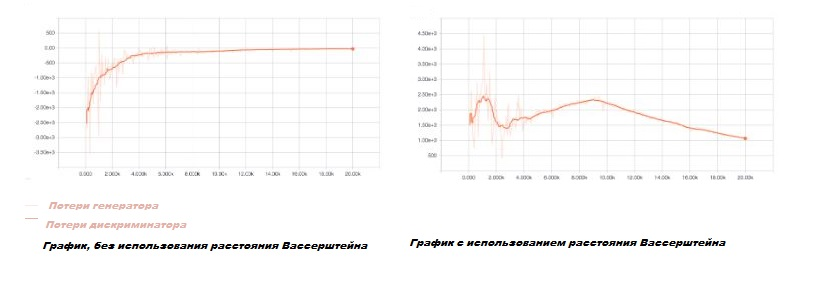
\includegraphics{img/1_10.jpg}
		\caption{Потери дискриминатора и генератора с использованием метода Вассерштейна и без.}}
\end{figure}

\newpage
Генератор $G(z; \theta_g)$ на каждой итерации обучения борется за инкремент значения потери, в свою очередь, для поддержки балансирования дискриминатор   $D(x; \theta_d)$ пытается декрементировать потерю, для генерации изображений неотличимых от оригинальных. Состязательный процесс между генератором и дискриминатором поддерживается особой структурой последнего, которая после каждого обновления значений, переданных генератором, имитирует подъем по градиентному спуску. В тоже время, при обучении генератора используется лишь метка, несущая значение потери, полученное от дискриминатора.

Для работы с цветовыми подсказками синтезируется эскиз для генератора в виде $G(z; z_{hint}; \theta_g)$, изменяется предварительный вывод дискриминатора на  $D(x; z_{hint}; \theta_d)$. Случайно поданное в сеть изображение z инициализирует карту изображения, которая представляет собой матрицу объектов входного канала сети. Матрица, заполненная случайно поданным изображением, инициализирует связь между входным каналом и дискриминатором.
Архитектура дискриминатора, работающего с цветовыми подсказками представлена на Рисунок 1.9.


\begin{figure}[ht!]
	\centering{ 
		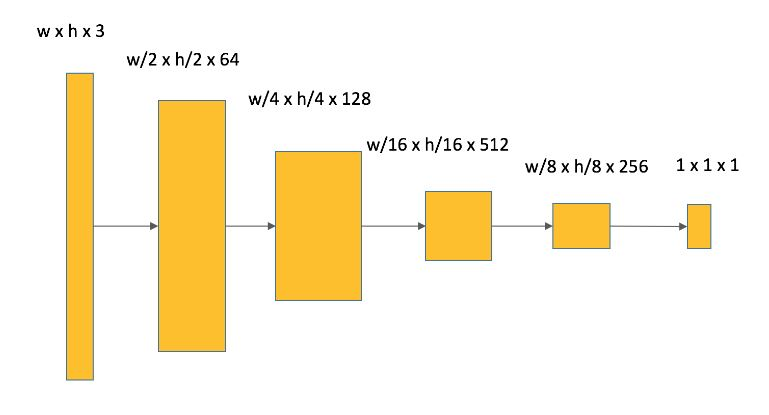
\includegraphics[width=0.5\textwidth]{img/1_11.jpg}
		\caption{Архитектура дискриминатора.}}
\end{figure}


\newpage
\section {Колоризация изображения с использованием цветного опорного.}
Данное решение закрашивает монохромное изображение используя опорное цветное изображение, график соответствия и метод квадратичного программирования. 
Работа алгоритма, разделенная по основным этапам, представлена на Рисунок 1.10.

\begin{figure}[ht!]
	\centering{ 
		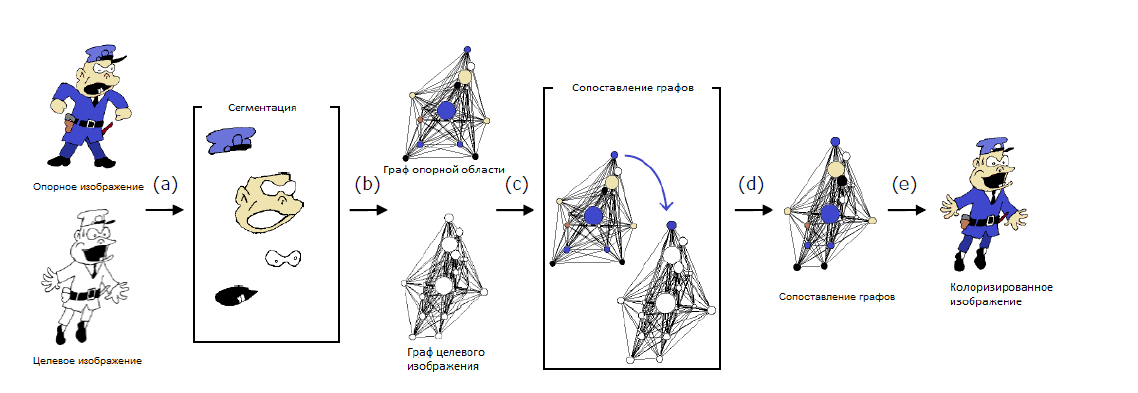
\includegraphics[width=1.0\textwidth]{img/3.png}
		\caption{Пример работы алгоритма}}
\end{figure}




Граф опорного изображения обозначим, как $G_r = (V_r , E_r)$, а граф целевого $G_t = (V_t , E_t)$, где $V$ - обозначает набор узлов, а $E$ - набор ребер. Решение определено, как матрица перестановок $X = (x_{i,j})_{N_r * N_t} \in {\{0,1\}}^{N_r*N_t}$. $N_t$ и $N_r$ обозначают число вершин целевого и опорного графов соответственно.


Когда $i$-ая область опорного изображения сопоставляется с $j$-ой областью целевого изображения для каждого столбца и строки матрицы $X$ должно выполняться:


\begin{equation}
\sum_{j} x_{i,j} = 1
\end{equation}

\begin{equation}
\sum_{i} x_{i,j} = 1
\end{equation}

Для реализации сопоставления графов $G_r$ и $G_t$ была введена функция стоимости $Q(i_1, j_1, i_2, j_2)$ :


\begin{equation}
Q(i_1, j_1, i_2, j_2) = D_{length} * D_{angle} * D_{area}
\end{equation}

\begin{equation}
D_{length} = \frac{||V_{i_1, i_2}| - |V_{j_1, j_2}||}{max(V_{i_1, i_2}, V_{j_1, j_2})}
\end{equation}

\begin{equation}
D_{angle} = \frac{1}{2} (1 - \frac{V_{i_1, i_2}*V_{j_1, j_2}}{|V_{i_1, i_2}||V_{j_1, j_2}|})
\end{equation}

\begin{equation}
D_{area} = \frac{|a_{i_1}a_{j_2} - a_{i_2}a_{j_1}|}{max(a_{i_1}, a_{j_2}, a_{i_2}, a_{j_2})}
\end{equation}



Три меры $ D_{length}, D_{angle}, D_{area} $ оценивают разницу между $(i_1, i_2); (j_1, j_2); (V_1, V_2)$. Если две пары имеют одинаковые относительные позиции, то стоимость переноса примет минимальное значение ( $Q(i_1, j_1, i_2, j_2) = 0$). Но если хотя бы одна из пар будет содержать фиктивный узел, то стоимость примет максимальное значение ( $Q(i_1, j_1, i_2, j_2) = 1$). 


Пример отношения между вершинами графов показан на Рисунок 1.11. 

\begin{figure}[ht!]
	\centering{ 
		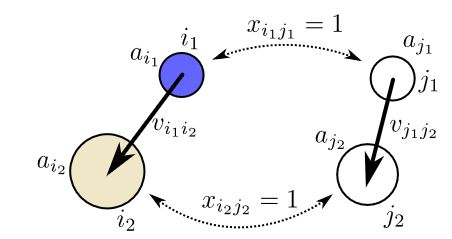
\includegraphics[width=0.5\textwidth]{img/1_12.jpg}
		\caption{Отношения между вершинами графов.}}
\end{figure}



Базируясь на этой идее, получаем что матрица $X$ может быть получена путем минимизации суммы 1.15 с ограничением. $\lambda_{min}$  - наименьшее собственное значение стоимости $Q$, $I$ - единичная матрица.

\begin{equation}
\sum_{i_1, j_1, i_2, j_2} Q(i_1, j_1, i_2, j_2) x_{i_1, j_1} x_{i_2, j_2} = X^t Q_x 
\end{equation}

\begin{equation}
min(X^t Q_x)  \Rightarrow min(X^t (Q_x - \lambda_{min} I))x + \lambda_{min} \sum_{i,j=1}^{N} x_{i,j} : x \in {\{0,1\}}^{N^2}
\end{equation}

\section{Сравнительный анализ методов.}
Вышеописанные методы имеют свои преимущества и недостатки. Они сведены в таблицу ниже, где "Метод №1" - это метод колоризации с использованием цветовых подсказок, а "Метод №2" - это метод колоризации с использованием опорного изображения, графика соответствия и методов квадратичного программирования.
\newpage
\begin{landscape}
\begin{table}[]
	\begin{tabular}{lll}
		\hline
		Метод №1 & Метод №2 & Параметры сравнения \\ \hline
		Загрузка целевого изображения. & \begin{tabular}[c]{@{}l@{}}Загрузка целевого изображения,\\ опорного изображения.\end{tabular} & Необходимость загрузки изображения \\
		Ожидание ввода цветовых подсказок. & - & Ожидание пользовательского ввода \\
		- & \begin{tabular}[c]{@{}l@{}}Требуется опорное изображение,\\ содержащее колоризованные \\ элементы целевого.\end{tabular} & Загрузка опорного изображения \\
		- & + & Использование графовых структур \\
		\begin{tabular}[c]{@{}l@{}}Хранение сгенерированных карт объектов,\\ передача этих матриц между слоями сети\end{tabular} & \begin{tabular}[c]{@{}l@{}}Хранит только 1 результирующую \\ матрицу.\end{tabular} & Хранение матриц \\
		\begin{tabular}[c]{@{}l@{}}Исправлены использованием расстояния \\ Вассерштейна.\end{tabular} & Не исправлены. (см Раздел 1.4.) & Недостатки, выявленные при колоризации \\
		\begin{tabular}[c]{@{}l@{}}Ресурсозатратный метод. Требует обучения\\ моделей.\end{tabular} & \begin{tabular}[c]{@{}l@{}}Обработка графовых структур. \\ Ресурсоемкий метод.\end{tabular} & Требование вычислительных ресурсов \\
		\begin{tabular}[c]{@{}l@{}}Медленный засчет счивания подсказок, \\ построения цветового распределения и \\ самого переноса соответсвия с применением \\ функции ошибки.\end{tabular} & \begin{tabular}[c]{@{}l@{}}Быстрее метода №1. Так как выставляет\\ цветовое соотвествие сразу, используя \\ опорный граф и методы\\ квадратичного программирования.\end{tabular} & Скорость работы предложенного метода
	\end{tabular}
\end{table}
\end{landscape}

Ниже приведены примеры работы "Метода №1" и "Метода №2". Так же представлен случай, описывающий недостатки колоризации вторым методом. (см. Рисунок 1.12)

\begin{figure}[ht!]
	\centering{ 
		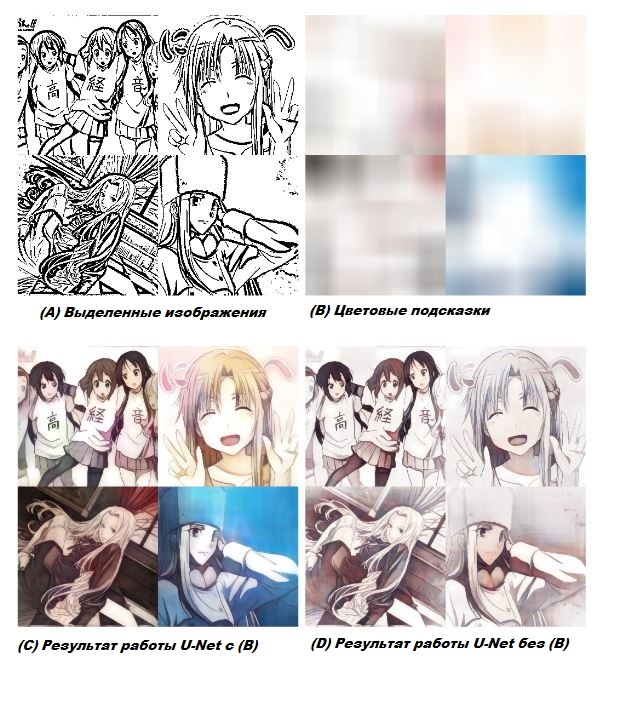
\includegraphics[width=0.7\textwidth]{img/1_9.jpg}
		\caption{Пример работы "Метод №1".}}
\end{figure}

Как можно видеть из Рисунок 1.12 данный метод, может колоризировать монохромное изображение также без ввода цветовых подсказок, дискриминатор лишь примет значение у генератора цветового распределения, которое уже было встречено в процессе обучения на наборе данных. Если же добавить цветовые подсказки, то результат изменится, но также увеличится и время работы метода, так как начнется ресурсозатратная гонка между генератором и дискриминатором, описанная выше и представленная на графике Рисунок 1.7.


\begin{figure}[ht!]
	\centering{ 
		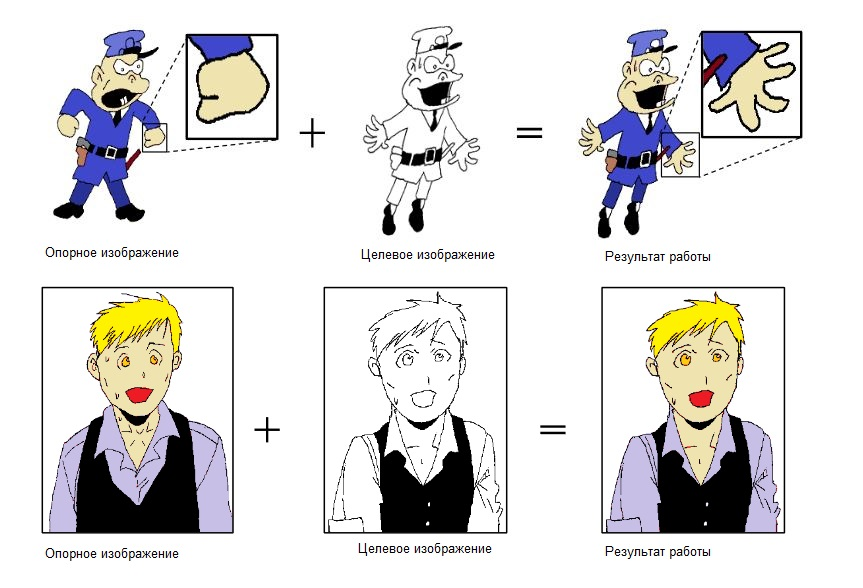
\includegraphics[width=0.7\textwidth]{img/1_13.jpg}
		\caption{Примеры работы "Метод №2".}}
\end{figure}

\begin{figure}[ht!]
	\centering{ 
		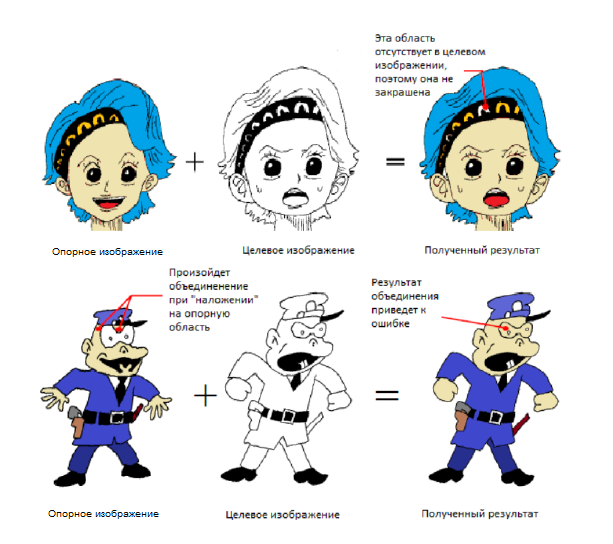
\includegraphics[width=0.7\textwidth]{img/4.png}
		\caption{Недостатки  работы "Метод №2".}}
\end{figure}

Как видно из примеров работы, представленных на Рисунок 1.13, данный способ колоризации справляется с решением поставленной задачи в случае, если число узлов графа опорного изображения совпадает с числом узлов графа, целевого.


 На примерах из Рисунок 1.14 видно, что в противном случае область, не проинициализированная узлом на графе опорного изображения, остается не закрашенной. Если же область была проинициализирована узлом на графе опорного изображения, а на графе целевого изображения отсутсвует узел, отвечающий за соответствующую область, то происходит сильное искажение целевой области относительно используемой опорной, что приводит к неверному результату работы.